\title{Midterm 3 for Algebra-Based Physics-1: Mechanics (PHYS135A-01)}
\author{Dr. Jordan Hanson - Whittier College Dept. of Physics and Astronomy}
\date{November 19th, 2017}
\documentclass[10pt]{article}
\usepackage[a4paper, total={18cm, 27cm}]{geometry}
\usepackage{outlines}
\usepackage[sfdefault]{FiraSans}
\usepackage{graphicx}

\begin{document}
\maketitle
\small
\section{Equation and Constants}
Definition of the radian: $s = r \theta$ \\
Angular velocity (change in radians per unit time): $\omega = \Delta \theta/\Delta t$ \\
Angular velocity (change in $\omega$ per unit time): $\alpha = \Delta \omega/\Delta t$ \\
Tangential velocity: $v = r\omega$ \\
Tangential acceleration $a = r\alpha$ \\
Centripetal acceleration: $a_c = r\omega^2 = v^2/r$ \\
Centripetal force: $F_c = m a_c$ \\
Newton's Law of Gravity: $F_G = G m_1 m_2 / r^2$, $G = 6.674\times 10^{-11}$ N m$^2$ kg$^{-2}$ \\
Kepler's 3rd Law (explicit): $r^3/T^2 = \frac{G}{4\pi^2} M$, where $M$ is the mass of the central body. \\
Kepler's 3rd Law (scaling): $r_1^3/T_1^2 = r_2^3/T_2^2 = const$ \\
Definition of Work: $W = \vec{F} \cdot \vec{d} = Fd\cos\theta$ \\
Definition of kinetic energy: $KE = \frac{1}{2} mv^2$ \\
Work-Energy theorem: $W = \Delta KE$ \\
Definition of gravitation potential energy: $U = mgh$ \\
\textbf{Conservation of energy}: $KE_i + U_i = KE_f + U_f$

\section{Rotational Kinematics and Dynamics}
\begin{enumerate}
\item Express the following angles in radians: (a) $45^{\circ}$ (b) $30^{\circ}$ (c) $215^{\circ}$ \\ \vspace{1.75cm}
\item A man spins a grindstone to sharpen a knife, and can accelerate the grindstone with a foot pedal.  Suppose the grindstone has a radius $r=6$ cm, and is spinning initially at 120 rpm.  (a) What is the angular velocity in rad/sec? (b) What is the tangential velocity, $v$? (c) If he presses the foot pedal and the angular velocity increases from 120 rpm to 240 rpm in 2 seconds, what is the angular acceleration? \\ \vspace{2cm}
\item A centrifuge for separating dissolved solids in a liquid is shown in Fig. \ref{fig:cent}.  The tangential velocity is $v=6$ m/s, and the radius is $r=3$ cm.  (a) What is the angular velocity? (b) What is the centripetal acceleration at the location of $m$? (c) How many g's is the centripetal acceleration?
\begin{figure}[ht]
\centering
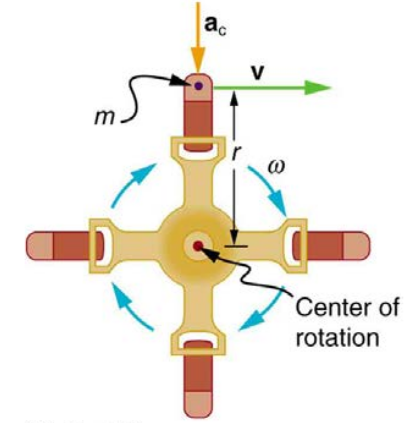
\includegraphics[width=0.2\textwidth]{figures/centrifuge.png}
\caption{\label{fig:cent} A centrifuge undergoes uniform circular motion, with tangential velocity $v$ and radius $r$.}
\end{figure} \\ \vspace{2cm}
\item A car traveling along a banked curve with radius $r$ is illustrated in Fig. \ref{fig:car}.  (a) Show that if the net force is zero as the car goes through this curve of radius $r$, that the speed of the car is $v = \sqrt{rg\tan\theta}$. (b) What is $v$, if $r=500$ m, $g\approx 10$ m/s$^2$, and $\theta = 15^{\circ}$?
\begin{figure}[ht]
\centering
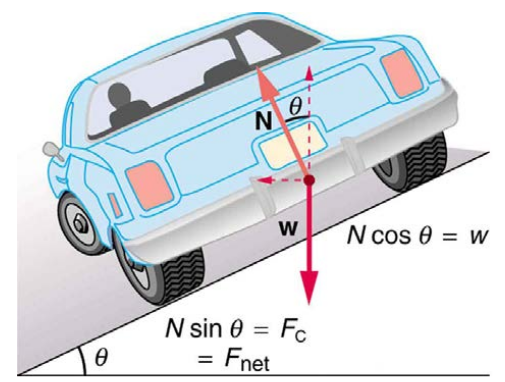
\includegraphics[width=0.25\textwidth]{figures/car.png}
\caption{\label{fig:car} A vehicle travels along a banked curve, hugging the road.}
\end{figure} \\ \vspace{1cm}
\end{enumerate}
\section{Newton's Law of Gravity}
\begin{enumerate}
\item Consider Fig. \ref{fig:planet}, in which a planet orbits a star.  If $a$ is the acceleration due to gravity \textit{on the surface} of the planet, show that $a = GM_p/d^2$, where $G$ is Newton's constant (\textit{Hint: set the weight vector equal to Newton's law of gravity}).  (b)  What is $M_p$, if $a=8.1$ m/s$^2$, and $d = 5500$ km? (c) Use Kepler's 3rd law to show that if the period of the orbit is $T$, that $M_S = 4\pi^2 b^3/(GT^2)$. (d) If $b = 6 \times 10^{11}$ m (about 4 AU), and $T = 4$ years, what is $M_S$? \\ \vspace{2cm}
\begin{figure}[hb]
\centering
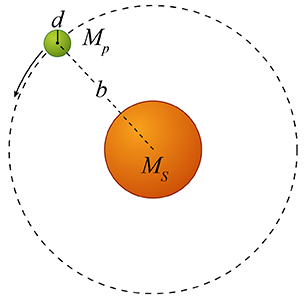
\includegraphics[width=0.25\textwidth]{figures/planet.png}
\caption{\label{fig:planet} A planet of mass $M_P$ and radius $d$ orbits a star of mass $M_S$ at an orbital radius $b$.}
\end{figure} \\ \vspace{0.5cm}
\item What is the orbital period of Jupiter, $T_N$ (in years), if the orbital radius of Jupiter, $r_N$, is 5 AU? (Recall that $T_{Earth} = 1.0$ year and $r_{Earth} = 1.0$ AU, and that this is a scaling problem). \\ \vspace{1cm}
\end{enumerate}
\section{Work and the Work-Energy Theorem}
\begin{enumerate}
\item If we place a force $\vec{F} = 2\hat{i} + 2\hat{j}$ N on an object that is displaced by $\vec{d} = 3\hat{j}$ m, what is the work $W$? \\ \vspace{0.75cm}
\item (a) If a person throws a 0.145 kg baseball at $v=8$ m/s, what is the kinetic energy of the baseball?  (b) If a person drops a 0.145 kg baseball from a building that is 40 m tall, what is the final speed of the baseball? \\ \vspace{1cm}
\item Consider Fig. \ref{fig:coaster}.  The cars star with no initial velocity, but have a mass of 300 kg.  (a) What is the initial kinetic energy? (b) What is the initial potential energy? (c) What is the final gravitational potential energy? (d) What is the final kinetic energy? (e) What is the final velocity?
\begin{figure}[ht]
\centering
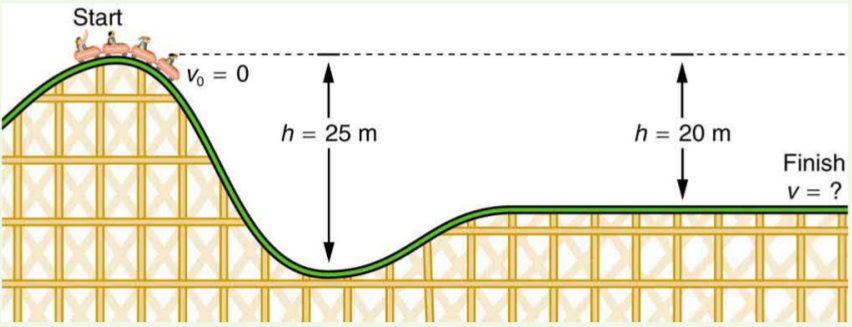
\includegraphics[width=0.5\textwidth]{figures/coaster.png}
\caption{\label{fig:coaster} A roller coaster starts with no initial velocity, but ends with velocity $v$.}
\end{figure}
\end{enumerate}
\end{document}